\chapter[Melhorias Propostas]{Melhorias Propostas}
\label{chap:melhorias}

	\section[Definição]{Definição}
	\label{sec:melhorias_definicao}

		A produção de produtos/serviços é uma questão importante no cotidiano. É comum as pessoas estarem ora dentro de um processo de produção ora clientes desse processo de produção. Contudo, existe uma caracterista imporante que culmina ambas as perspectivas, a qualidade. Para alcançar os objetivos de qualidade de uma produção não é nada fácil. Diversos critérios devem ser satisfatórios para uma qualificação de impacto, portanto, pode-se levantar 5 necessidades para um processo de qualidade. São elas:

		\begin{itemize}
			\item{Ser eficiente;}
			\item{Ser definido;}
			\item{Ser gerenciado;}
			\item{Ser medido;}
			\item{Ser controlado;}
		\end{itemize}

		Na prática, essas necessidades são muito difíceis de serem executadas paralelamente. Então, pra resolver essa dificuldade que surgiram os modelos de melhorias de processos, no qual consistem em uma estrutura genérica que descreve as fases, as atividades e os recursos necessários para um esforço de melhoria de um processo bem sucedido.

		Antes que se possa idealizar uma abordagem para o melhoramento de algumas operações, é preciso saber o quanto ela já é boa. A direção, urgência e prioridades de melhoramento serão determinadas parcialmente em razão de o atual desempenho de uma operação ser julgada como boa, ruim ou indiferente. Todas as operações produtivas, portanto, precisam de alguma forma de medida de desempenho, como pré-requisito para melhoramento. \cite{slack}

		O diagrama a seguir, ilustra a relação entre processo, medida de desempenho e melhorias para um processo.

		\newpage
		\begin{figure}[h]
			\centering
			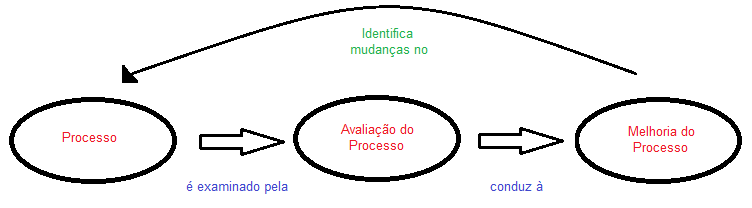
\includegraphics[scale=0.8]{melhoria1}
			\caption[Estratégia de Melhoria de um Processo]{Estratégia de Melhoria de um Processo}
			\label{fig:melhoria1}
		\end{figure}

		A partir da análise do gráfico anterior, percebe-se que um processo precisa ser avaliado antes do levantamento de qualquer proposta, servindo de parâmetro para comparação de "como está"  para "o que há de melhorar".

	\section[Aplicações]{Aplicações - 
\includegraphics{bobs2}}
	\label{sec:melhorias_aplicacoes}

		%A rede Bob's sofreu uma recente reestruturação e, infelizmente, não foi possível obter informações sobre. Portanto, as melhorias propostas aqui são ideias com base em dados quevão até 2011. 

		Por mais intenso que tenha sido o esforço para construção de melhorias expressivas, infelizmente com as pesquisas encontradas não é possível sugerir grandes mudanças, pois além de o processo de produção do \textbf{Bob's} ter sido avaliado em um âmbito macro, requerendo uma análise mais robusta e aprofundada para sugestões de melhorias interna à empresa, a rede passou por uma reestruturação recentemente, não permitindo adquirir mais informações a respeito. Abaixo se encontra uma figura que mostra o crescimento do \textbf{Bob's} entre 1996 e 2004 ilustrando os resultados oriundos da reestruturação ocorrida no período. 

		\begin{figure}[h]
			\centering
			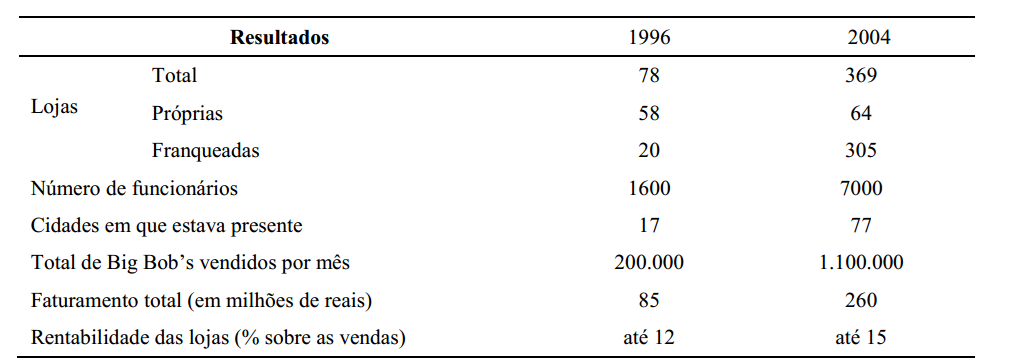
\includegraphics[scale=0.6]{tec4}
			\caption[Comparação dos resultados da rede Bob’s entre 1996 e 2004 ]{Comparação dos resultados da rede \textbf{Bob’s} entre 1996 e 2004. \cite{osman}}
			\label{fig:tec4}
		\end{figure}

		Para que ocorresse a reestruturação mostrada na figura acima, o \textbf{Bob’s}, mesmo perdendo para seus concorrentes nas redes sociais, como mostrado no capítulo \ref{chap:tecnologias} (\nameref{chap:tecnologias}), adotou medidas como reduzir a verticalização e focar na qualidade do serviço e produto final ao vender suas fábricas de hambúrguer, batata frita, sorvete e refresco, permitindo assim a obtenção dos mesmos já prontos e um maior foco nas suas campanhas de marketing, treinamento de funcionários e desenvolvimento de novos produtos, alcançando o crescimento citado anteriormente. 

		Por fim, após a análise da entrevista e de alguns artigos encontrados, foi possível propor algumas melhorias simplistas, identificadas para suprir algumas das necessidades de melhorias da empresa.

		A primeira melhoria proposta está em otimizar o atendimento nas franquias, aproveitando-se do aumento no uso de smartphones juntamente com seus aplicativos. Através da criação de um aplicativo, no qual o cliente faz todo o seu pedido e armazena seus dados como o número do cartão de crédito e, com isso, basta chegar no caixa e fazer a transferência dessas informações por meio da \emph{Near Field Communication} (NFC) ao aproximar o smartphone de uma máquina registradora de NFC. Com isso, a rede \textbf{Bob's} pode ter uma caixa registradora que capta o pedido do cliente e realiza o pagamento com a aproximação de um smartphone, utilizando comunicação por campo de proximidade. As vantagens dessa tecnologia tangem a facilidade e agilidade no atendimento ao cliente, além da segurança nas informações, uma vez que a NFC possui um protocolo de segurança para evitar a interceptação dos dados, no caso, o roubo de dados do cartão de credito do usuário (protocolo conhecido como \emph{Single Wire Protocol - SWP}).

		\begin{figure}[h]
			\centering
			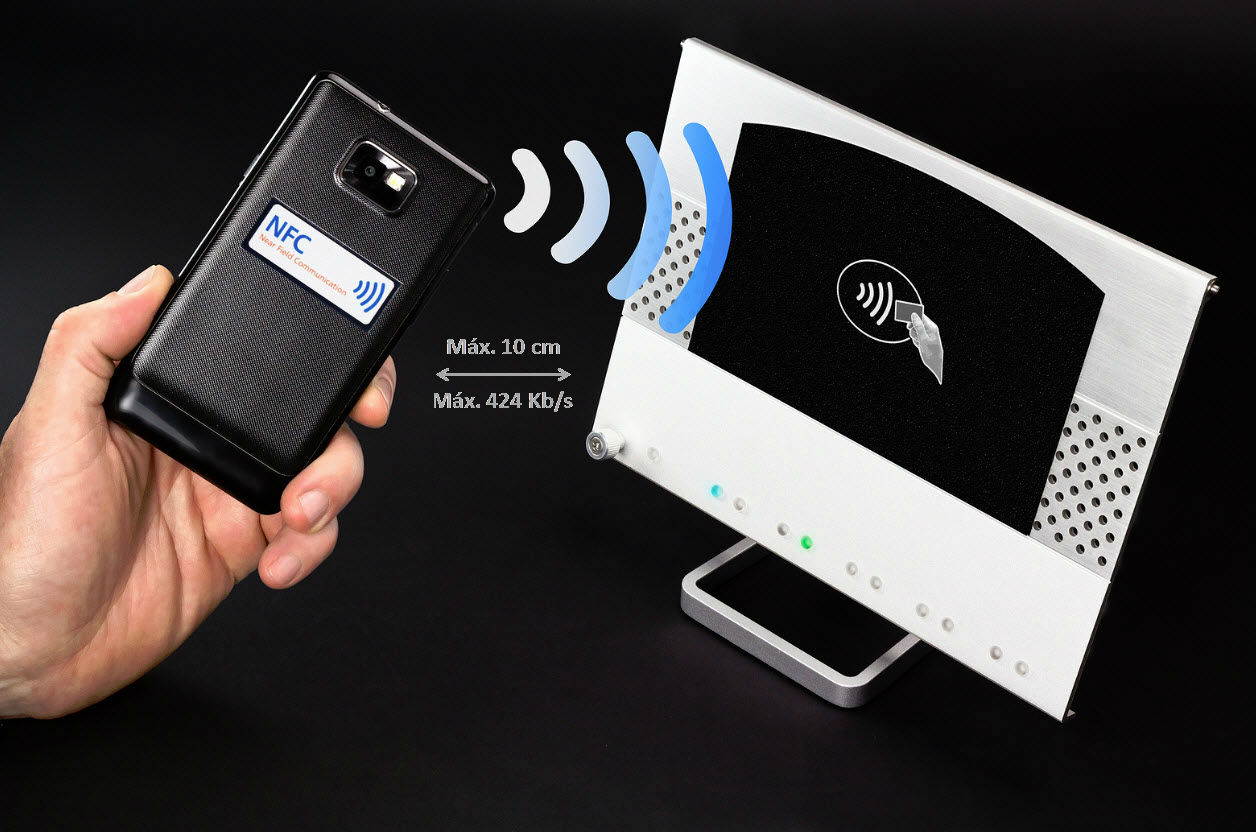
\includegraphics[scale=0.3]{melhoria2}
			\caption[Exemplo de utilização de NFC]{Exemplo de utilização de NFC}
			\label{fig:melhoria2}
		\end{figure}

		A segunda melhoria proposta está voltada na otimização do serviços de \emph{Delivery} do \textbf{Bob's} que consiste em colocar várias franquias voltadas exclusivamente para o delivery em vários lugares. Fazendo isso, além de expandir o alcance do \textbf{Bob's Delivery}, as franquias não necessitarão ter um espaço físico maior para atender a demanda, mas apenas o necessário para a produção dos produtos. Isso traria impactos positivos para a rede, pois o serviço possivelmente seria prestado em menos de 40 minutos devido ao aumento dos pontos de \emph{Delivery}. Além disso, pode-se aproveitar o uso do aplicativo sugerido anteriormente para o pagamentos dos pedidos realizados, e utilizando a tecnologia de GPS nas motos, pode-se ainda, informar ao cliente quanto tempo falta para seu produto chegar, a empresa vigiar a entrega e, em caso de acidente, facilitar o atendimento do socorro ao entregador e ao mesmo tempo agilizar um outro profissional para entrega. 

		\begin{figure}[h]
			\centering
			
\includegraphics[scale=0.5]{melhoria3}
			\caption[Bob's Delivery]{\textbf{Bob's Delivery}}
			\label{fig:melhoria3}
		\end{figure}